\section{System Overview}
\label{sec:system}

The system utilizes two identical 5-DoF SO-101 follower arms with a binary end-effector, each with position-controlled Feetech STS3215 servos exposed through HuggingFace LeRobot's~\cite{cadene2026lerobot} \texttt{SOFollower} bus interface. A single Intel RealSense D435i camera to one side of the arms provides a 640$\times$480 RGB stream at 30\,fps; only the color stream is used. 


\subsection{AprilTags \& Camera}

Six ArUco markers~\cite{garrido2014aruco} drawn from the AprilTag Tag16h5 dictionary~\cite{olson2011apriltag} label the scene:

\begin{itemize}
  \item Two 40 mm markers, one on each arm base, used for camera-to-base calibration
  \item Two 40 mm markers on the gripper fingers for runtime visual servoing
  \item Two 20 mm markers on opposite sides of the tray, separated by a known horizontal spacing (140 mm), which double as position references and as a tilt gauge via their relative height
\end{itemize}

Understanding the nomenclature of ArUco markers is important to select the appropriate markers for each task. AprilTags are categorized into groups, or "families" depending on their complexity and resistance to error as shown in Figure \ref{fig:apriltag picture}. Within "Tag16h5", the "16" refers to the number of pixels in the tag, in this case a 4 x 4 tag. The "h5" refers to the tag's resistance to error, or how many pixels would need to be perceived incorrectly before the tag is mistaken for a different tag. 

\begin{figure} [H]
    \centering
    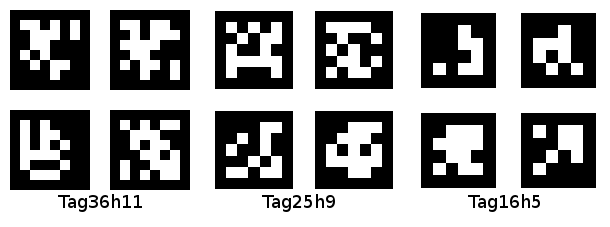
\includegraphics[width=1\linewidth]{subtex//images/AprilTags.png}
    \caption{Three different commonly used AprilTag families}
    \label{fig:apriltag picture}
\end{figure}

Generally, AprilTag families with less detail are used for applications at longer distances. Having less detail allows the tag to be easily discernible and therefore more reliable. Tags such as Tag36h11 contain more pixels as a 6 x 6 grid, and therefore have a higher resistance to error at h11. These tags are used for shorter ranges because they contain more detail and would be harder to percieve at long distances. 

Due to our size constraints, the simpler Tag16h5 AprilTags were used. The relative small scale of our setup simulates a long distance environment. Because our marker sizes were 20 mm for the tray and 40 mm for the end-effectors and we only needed 6 tags total, it was important for the tags to be as simple as possible so they could be read accurately.

These AprilTags were detected by a RealSense D435i Camera shown in Figure \ref{fig:camera}. Although the RealSense camera is capable of infrared (IR) stereo depth perception, it was not used due to noise and unreliability. Instead, steady RGB footage at 30 Hz was utilized. Both robot arms shared context through this camera, but because they run in separate threads, this simulates having two cameras placed in the same position. Two cameras would have been preferred for added generalizability, but resource constraints prohibited this augmentation.

\begin{figure} [H]
    \centering
    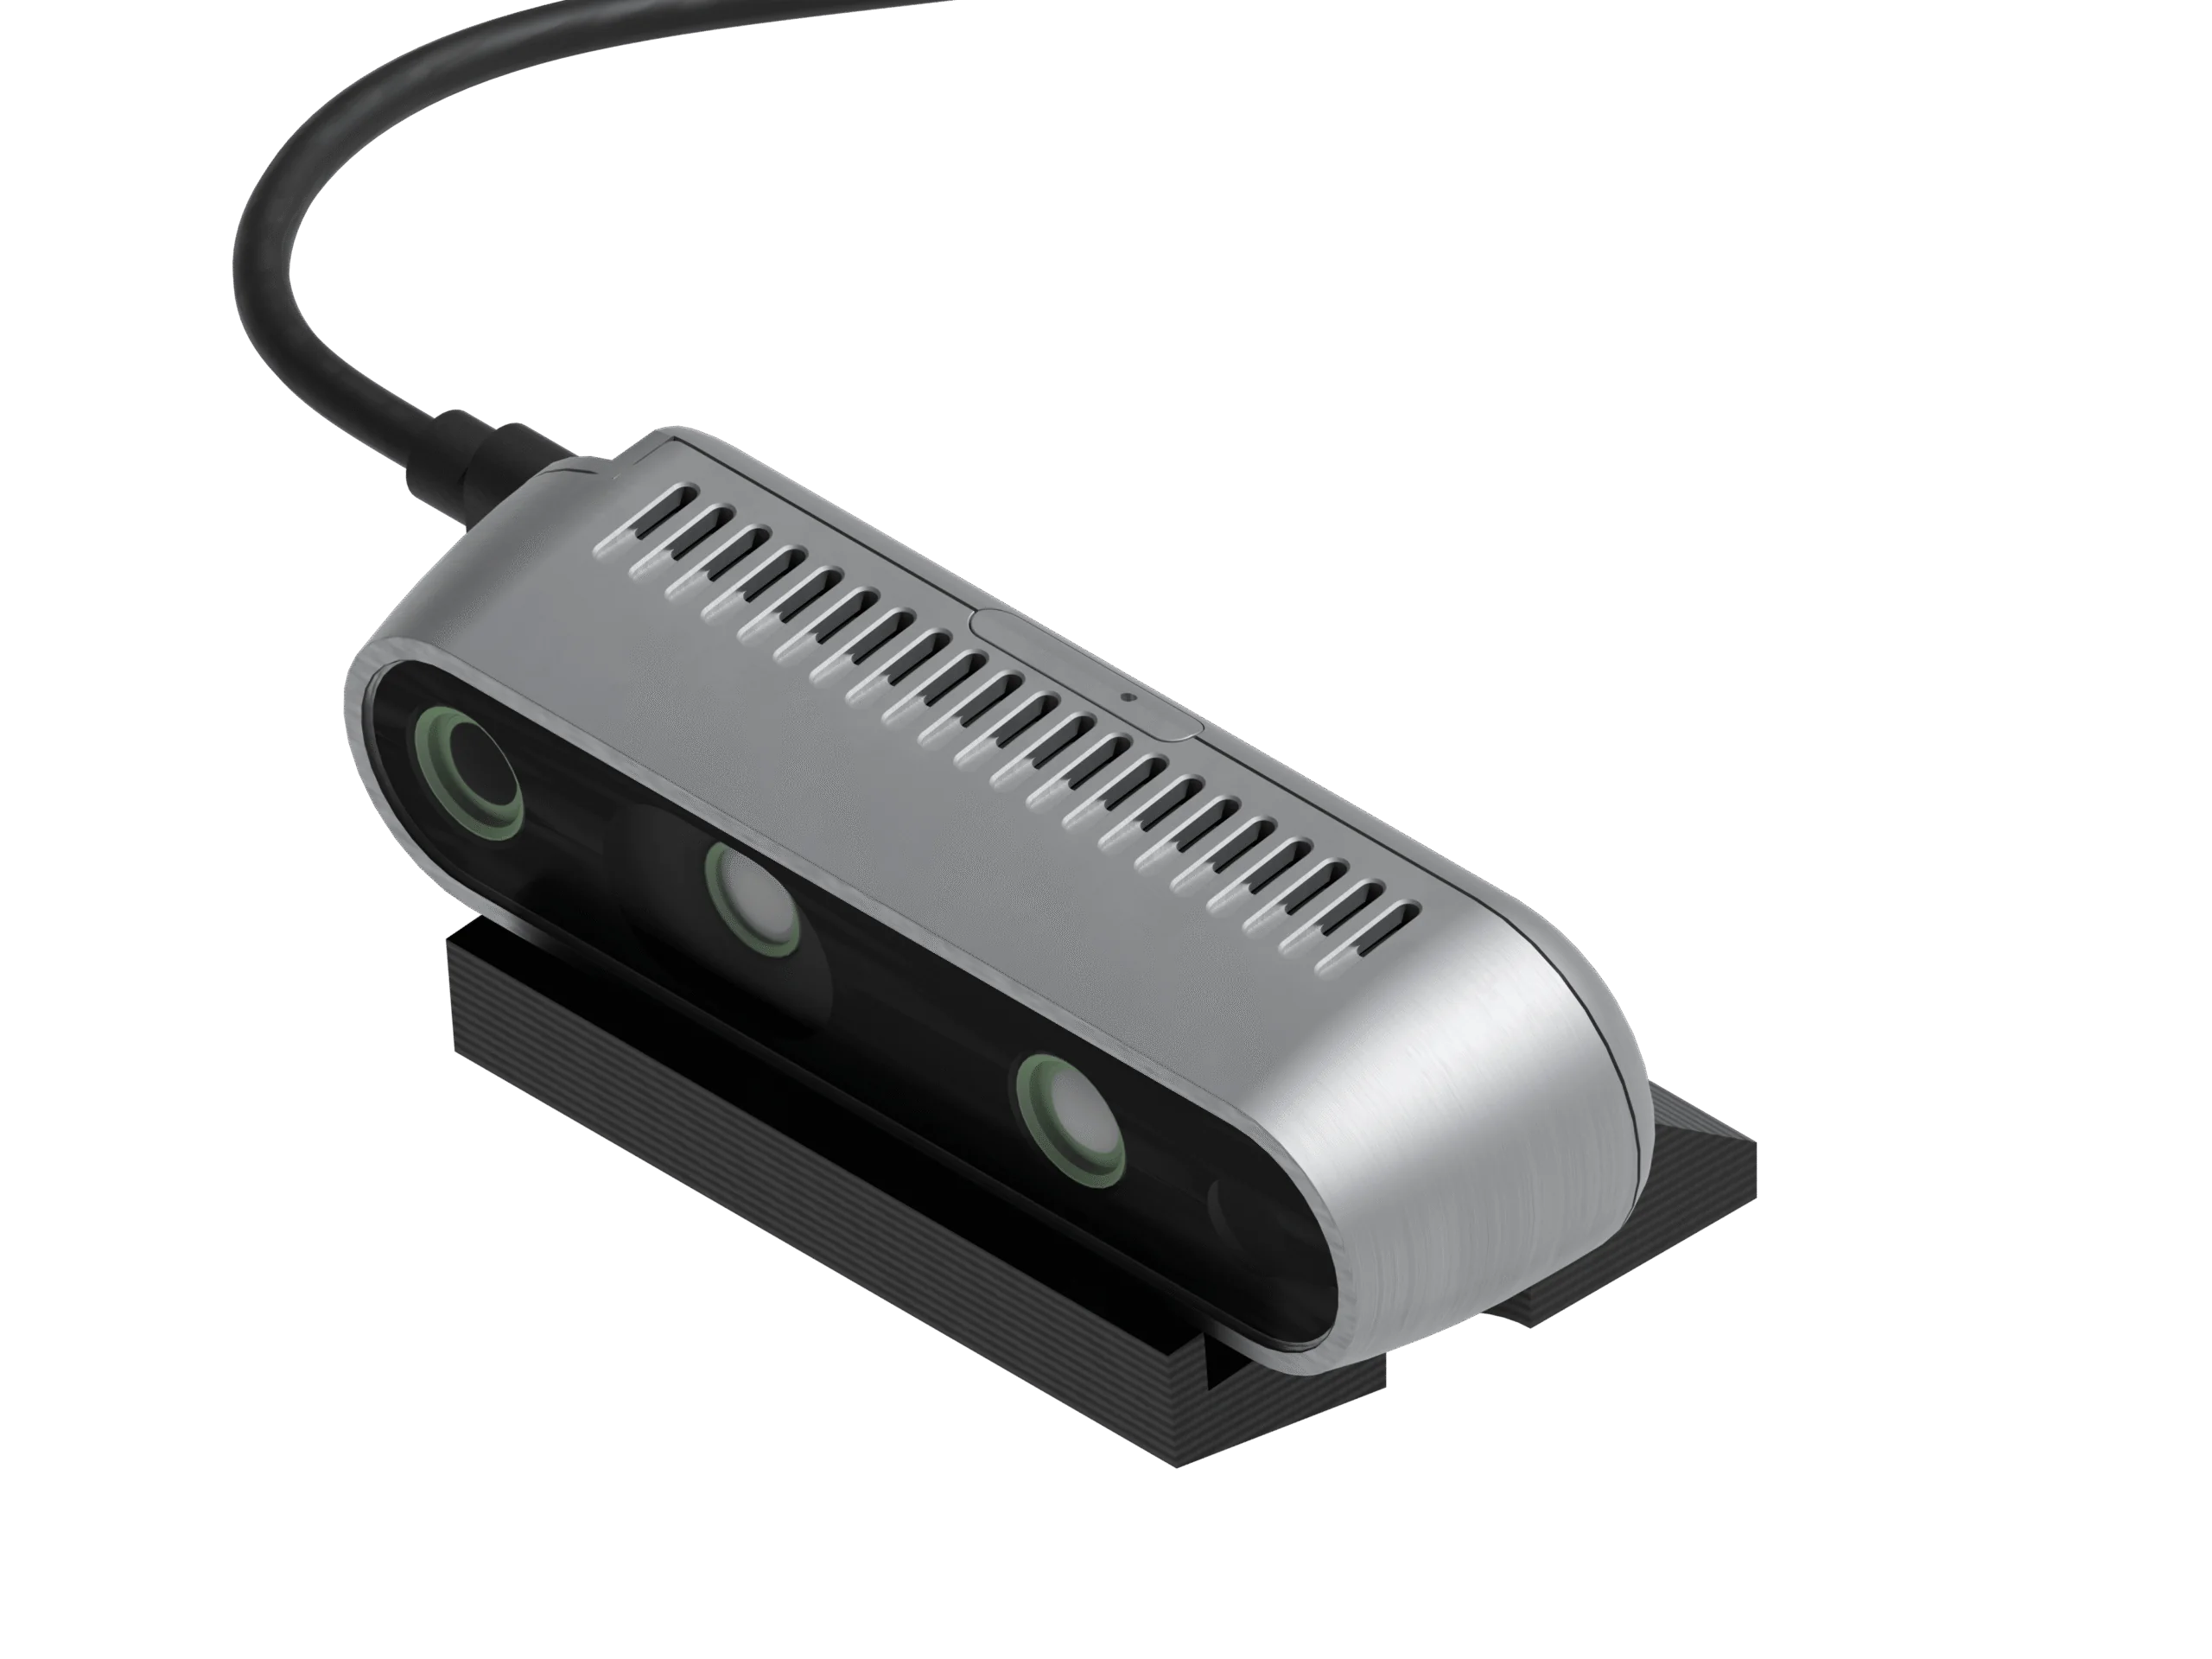
\includegraphics[width=1\linewidth]{subtex//images/camera.png}
    \caption{Realsense D435i Camera}
    \label{fig:camera}
\end{figure}




\subsection{Hardware Modifications}
The Lerobot SO-101, shown in Figure \ref{fig:unmodified lerobot arm} below, is an open source platform and was not immediately amenable for this application. Namely, the end-effector assembly and range of motion were not suited for bimanual tray lifting and translating. The team used Fusion 360 AutoDesk CAD to modify the design, and a Bambu X1E FDM 3D printer to manufacture the parts. 


\begin{figure} [h]
    \centering
    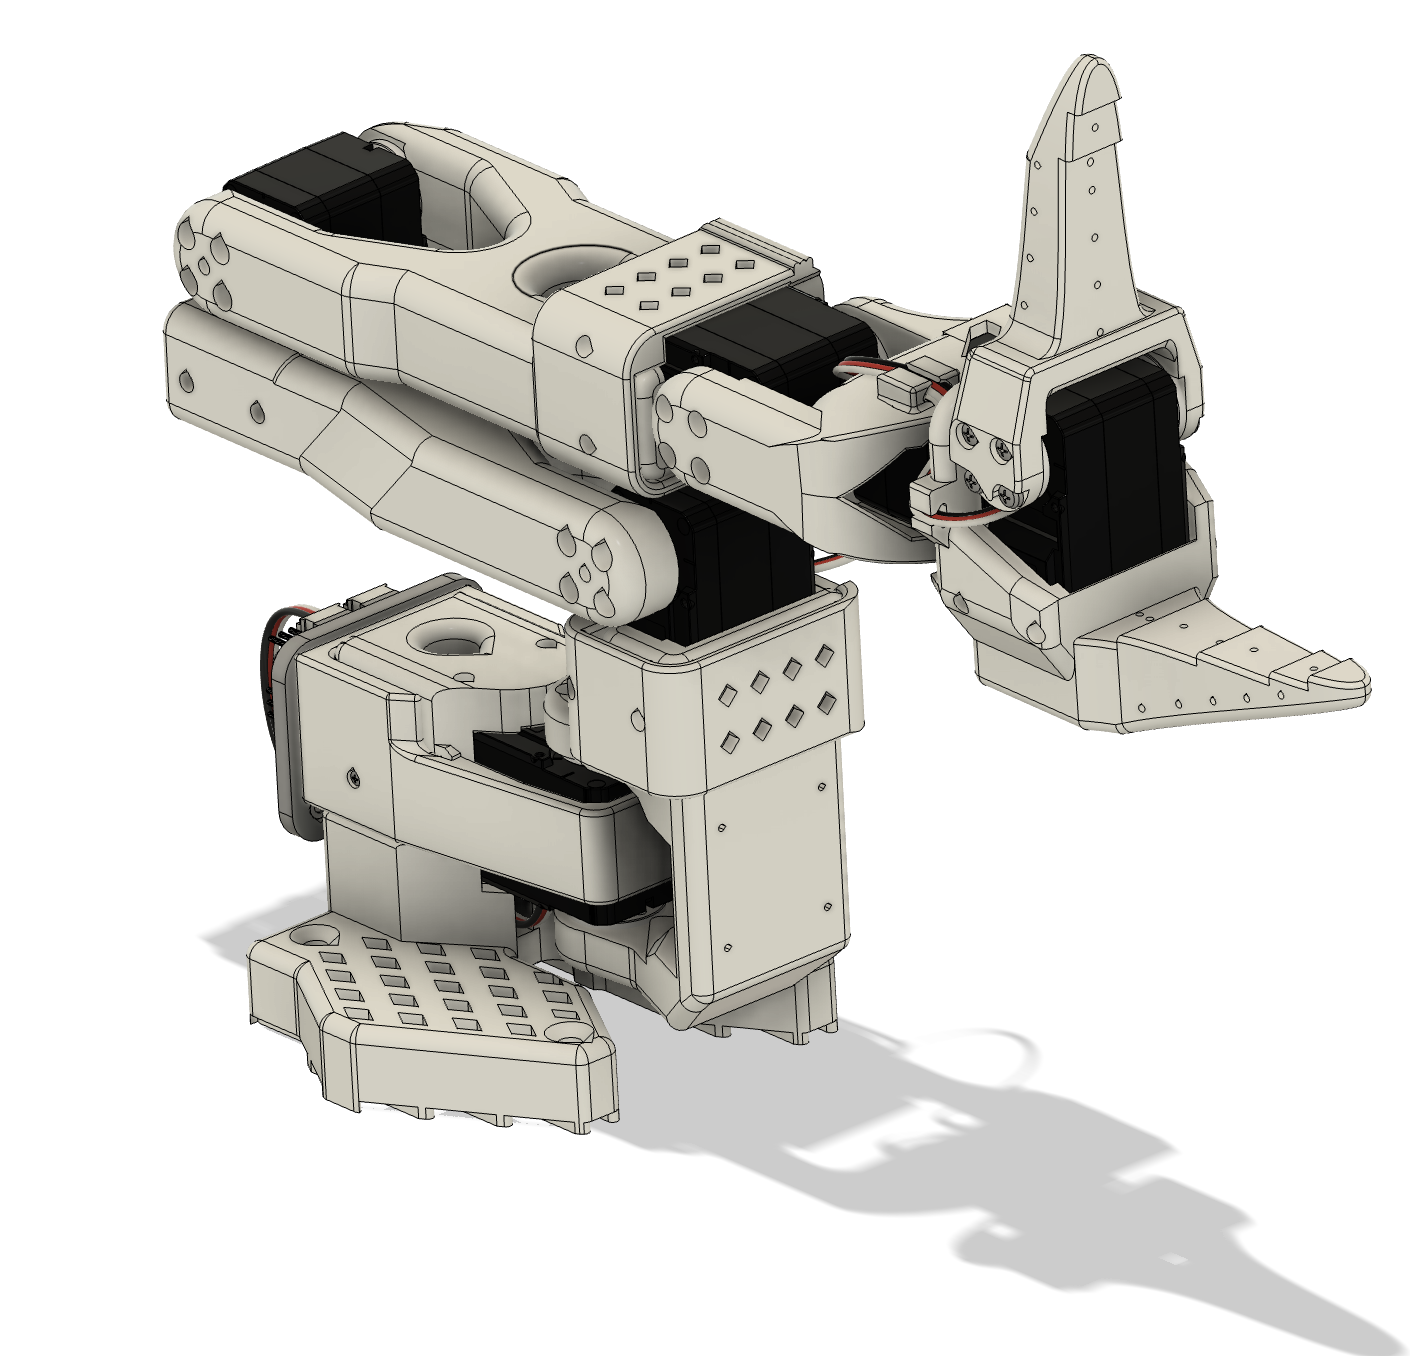
\includegraphics[width=1\linewidth]{subtex//images/original_lerobot.png}
    \caption{Unmodified Lerobot Arm}
    \label{fig:unmodified lerobot arm}
\end{figure}

The original "Finger-Tips" end-effector assembly shown in Figure \ref{fig:unmodified lerobot arm} was sub-optimal for our application. The swinging motion proved space-inefficient for a simplistic binary open-close program. The "Finger-Tips" were also originally printed in polylactic acid (PLA), a cost-effective but britle and unforgiving material for this application. Instead, another open source design \cite{so101grabcad} was used. This design features linearly translating grippers actuated through a gear and set of racks. A new servo casing and gear was designed to fit the STS3215 servo motor as shown in Figure \ref{fig:modified_end_effector_assembly}.




\begin{figure}[H]
    \centering
    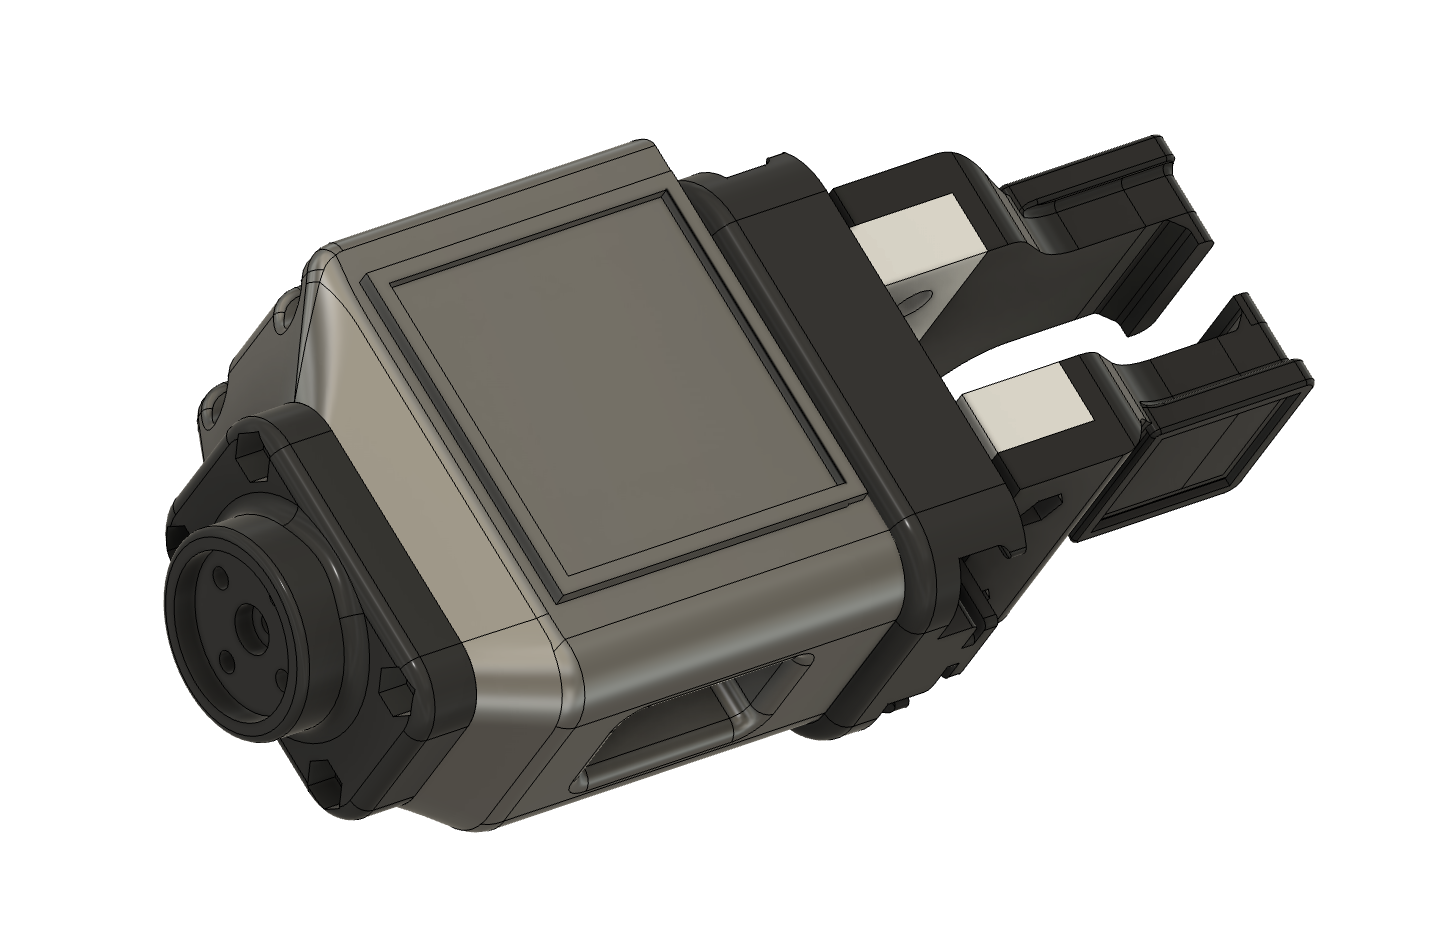
\includegraphics[width=1\linewidth]{subtex/images/gripper.png}
    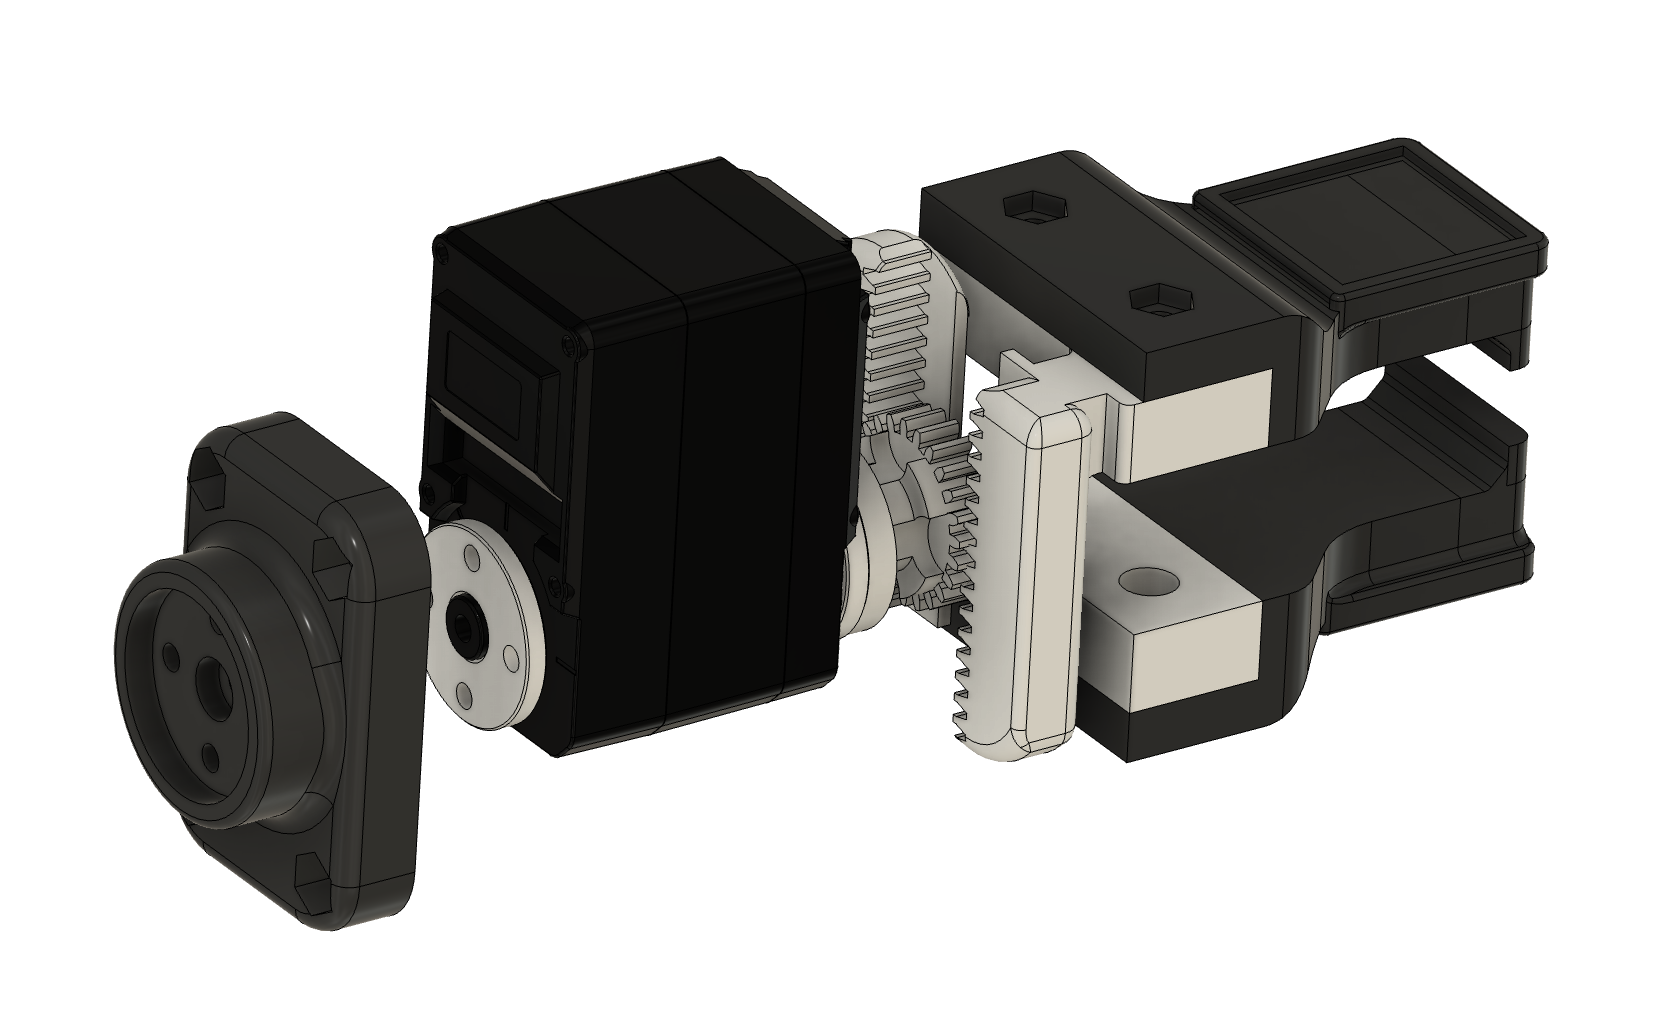
\includegraphics[width=1\linewidth]{subtex/images/exploded_end_effector.png}
    \caption{Modified End-Effector Assembly}
    \label{fig:modified_end_effector_assembly}
\end{figure}


The new design splits the individual end-effectors into two components, allowing for different materials. Thermoplastic polyurethane (TPU), a flexible filament, was used for the tips. This added flexibility was crucial in dampening excessive movement error during operation and program iteration. 

Another limiting design characteristic of the initial design was their range of motion when lifting the tray vertically at an extended distance. The robot end-effector would reach a ceiling and begin to rotate to achieve additional vertical range. This induced rotation would lead to task failure. To compensate, two modifications were made. First, the robot arm base was extended by 3 cm vertically, with the new design highlighting this modification shown in Figure \ref{fig:modified base picture}. Second, the "Bicep" arm, or lower robot arm, was also extended by 3 cm, again shown in Figure \ref{fig:bicep_picture}.

\begin{figure} [H]
    \centering
    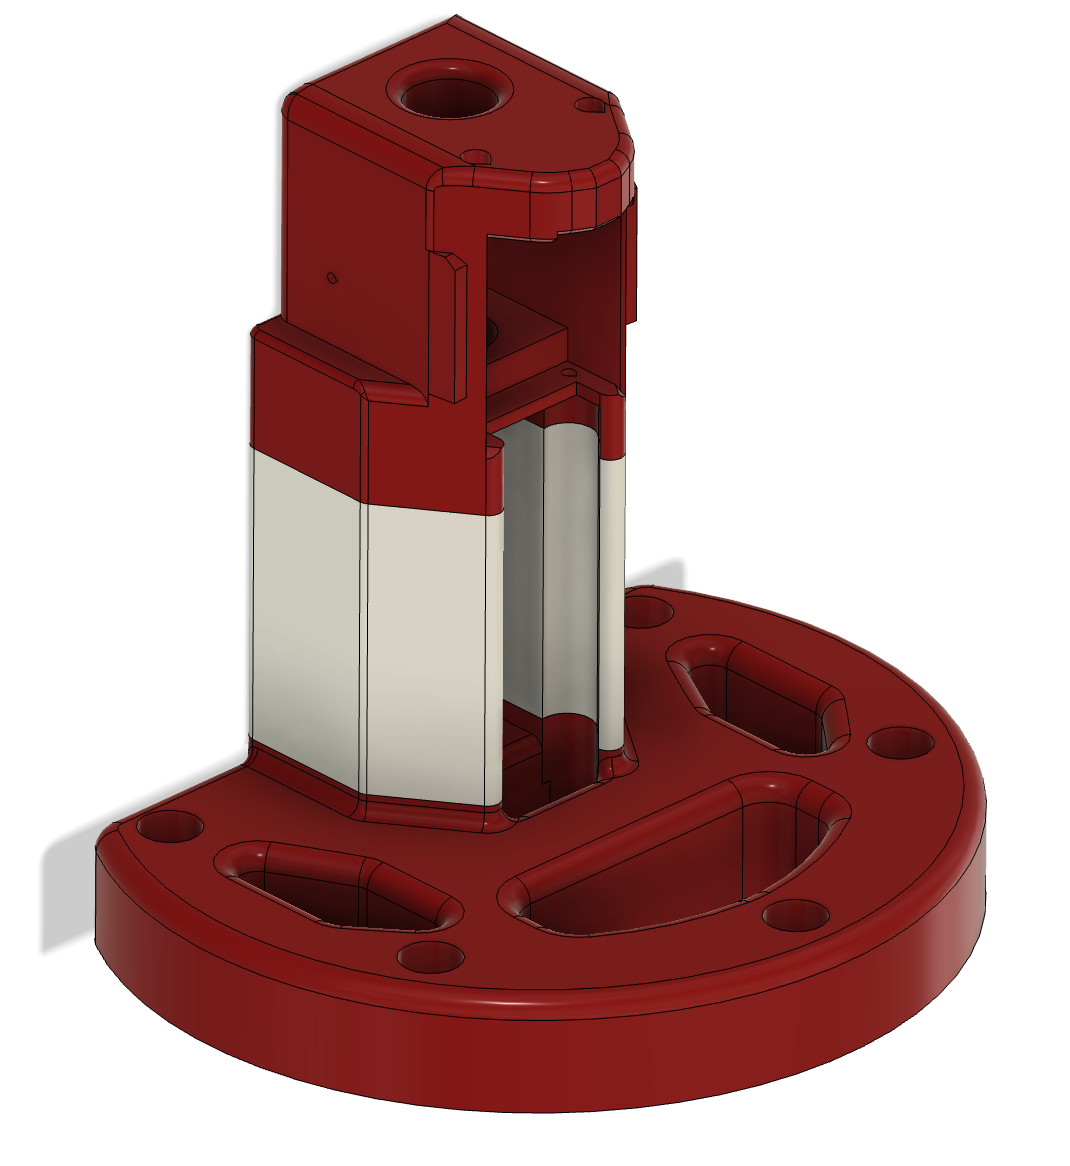
\includegraphics[width=1\linewidth]{subtex/images/base_modified.png}
    \caption{Modified Base}
    \label{fig:modified base picture}
\end{figure}

\begin{figure} [H]
    \centering
    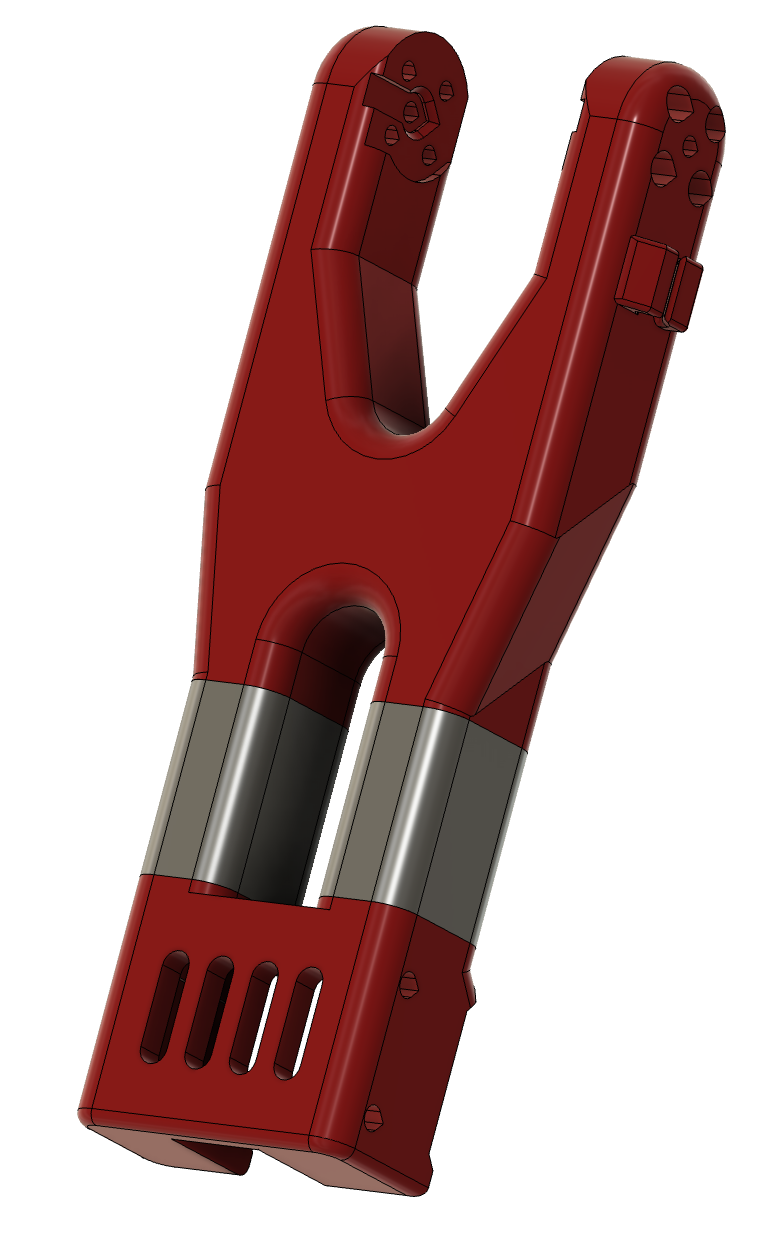
\includegraphics[width=.8\linewidth]{subtex/images/extended_bicep.png}
    \caption{Extended "Bicep" Arm}
    \label{fig:bicep_picture}
\end{figure}


\subsection{Tray}

The tray shown in Figure \ref{fig:tray} was designed from scratch. Printed from PLA, it features two AprilTag slots for 20 mm markers, as well as 10 mm wide handles raised 65 mm high. The tray itself is 150 mm in length and 75 mm in depth. While the tray design and assembly posed no significant problems towards the final task, a potential improvement, although less generalizable, would be to make a circular insert in the center to place the glass. This would prevent any lateral sliding in the case of jitter or small tilts.


\begin{figure} [H]
    \centering
    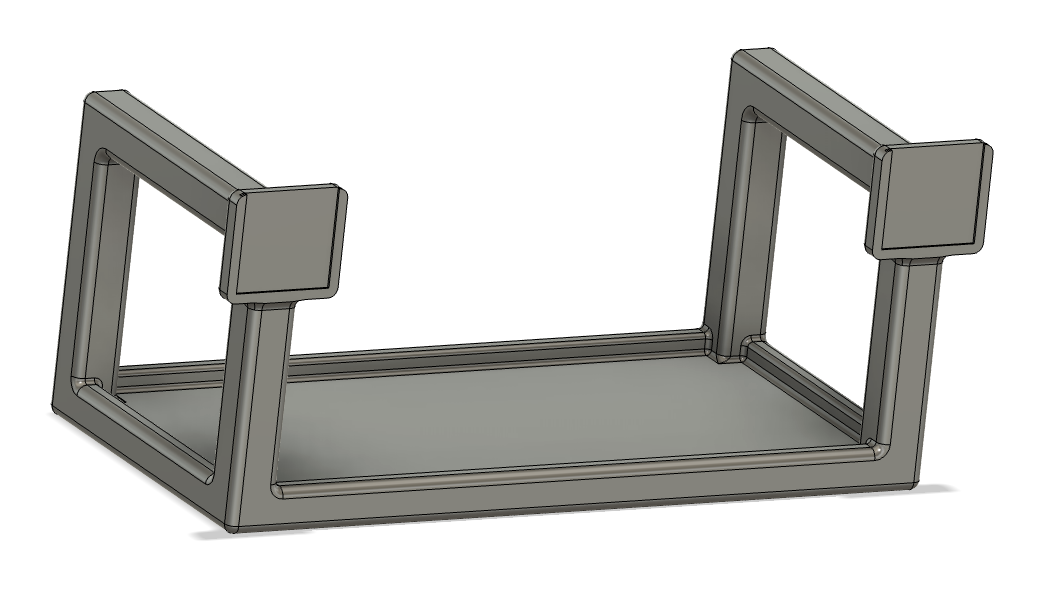
\includegraphics[width=1\linewidth]{subtex//images/tray.png}
    \caption{Custom Tray}
    \label{fig:tray}
\end{figure}



